% Soubory musí být v kódování, které je nastaveno v příkazu \usepackage[...]{inputenc}

\documentclass[%        Základní nastavení
  %draft,    				  % Testovací překlad
  12pt,       				% Velikost základního písma je 12 bodů
	t,                  % obsah slajdů bude vždy začínat od shora (nebude vertikálně centrovaný)
	aspectratio=1610,   % poměr stran bude 16:10 (všechny projektory v učebnách na Technické 12 Brno),
	                    % další volby jsou 43, 149, 169, 54, 32.
	unicode,						% Záložky a informace budou v kódování unicode
]{beamer}				    	% Dokument třídy 'zpráva', vhodná pro sazbu závěrečných prací s kapitolami
%\usepackage{etex}

\usepackage[utf8]		  % Kódování zdrojových souborů je v UTF-8
	{inputenc}					% Balíček pro nastavení kódování zdrojových souborů
	
\usepackage{graphicx} % Balíček 'graphicx' pro vkládání obrázků
											% Nutné pro vložení logotypů školy a fakulty

\usepackage[          % Balíček 'acronym' pro sazby zkratek a symbolů
	nohyperlinks				% Nebudou tvořeny hypertextové odkazy do seznamu zkratek
]{acronym}						
											% Nutné pro použití prostředí 'acronym' balíčku 'thesis'

%% Balíček hyperref je volán třídou beamer automaticky, proto není třeba následujícího kódu:
%\usepackage[
%	breaklinks=true,		% Hypertextové odkazy mohou obsahovat zalomení řádku
%	hypertexnames=false % Názvy hypertextových odkazů budou tvořeny
%											% nezávisle na názvech TeXu
%]{hyperref}						% Balíček 'hyperref' pro sazbu hypertextových odkazů
%											% Nutné pro použití příkazu 'nastavenipdf' balíčku 'thesis'

\usepackage{cmap} 		% Balíček cmap zajišťuje, že PDF vytvořené `pdflatexem' je
											% plně "prohledávatelné" a "kopírovatelné"

%\usepackage{upgreek}	% Balíček pro sazbu stojatých řeckých písmem
											%% např. stojaté pí: \uppi
											%% např. stojaté mí: \upmu (použitelné třeba v mikrometrech)
											%% pozor, grafická nekompatibilita s fonty typu Computer Modern!

%\usepackage{amsmath} %balíček pro sabu náročnější matematiky

\usepackage{booktabs} % Balíček, který umožňuje v tabulce používat
                      % příkazy \toprule, \midrule, \bottomrule

%%%%%vlastni balicky
\usepackage{makecell}
\usepackage{siunitx}
\sisetup{output-decimal-marker = {,}}
\DeclareSIUnit\LSB{LSB}
\sisetup{
  inter-unit-product=\ensuremath{{\cdot}},
%  tight-spacing=true,
}
\usepackage{subfigure}
\usepackage{tablefootnote}
\usepackage{amsmath}
\usepackage[thinc]{esdiff}


%%%%%%%%%%%%%%%%%%%%%%%%%%%%%%%%%%%%%%%%%%%%%%%%%%%%%%%%%%%%%%%%%
%%%%%%      Definice informací o dokumentu             %%%%%%%%%%
%%%%%%%%%%%%%%%%%%%%%%%%%%%%%%%%%%%%%%%%%%%%%%%%%%%%%%%%%%%%%%%%%

% V tomto souboru se nastavují téměř veškeré informace, proměnné mezi studenty:
% jméno, název práce, pohlaví atd.
% Tento soubor je SDÍLENÝ mezi textem práce a prezentací k obhajobě -- netřeba něco nastavovat na dvou místech.

\usepackage[
%%% Z následujících voleb jazyka lze použít pouze jednu
  czech-english,		% originální jazyk je čeština, překlad je anglicky (výchozí)
  %english-czech,	% originální jazyk je angličtina, překlad je česky
  %slovak-english,	% originální jazyk je slovenština, překlad je anglicky
  %english-slovak,	% originální jazyk je angličtina, překlad je slovensky
%
%%% Z následujících voleb typu práce lze použít pouze jednu
  semestral,		  % semestrální práce (výchozí)
  %bachelor,			%	bakalářská práce
  %master,			  % diplomová práce
  %treatise,			% pojednání o disertační práci
  %doctoral,			% disertační práce
%
%%% Z následujících voleb zarovnání objektů lze použít pouze jednu
%  left,				  % rovnice a popisky plovoucích objektů budou zarovnány vlevo
	center,			    % rovnice a popisky plovoucích objektů budou zarovnány na střed (vychozi)
%
]{thesis}   % Balíček pro sazbu studentských prací


%%% Jméno a příjmení autora ve tvaru
%  [tituly před jménem]{Křestní}{Příjmení}[tituly za jménem]
% Pokud osoba nemá titul před/za jménem, smažte celý řetězec '[...]'
\author{Marek}{Coufal}

%%% Identifikační číslo autora (VUT ID)
\butid{240598}

%%% Pohlaví autora/autorky
% (nepoužije se ve variantě english-czech ani english-slovak)
% Číselná hodnota: 1...žena, 0...muž
\gender{0}

%%% Jméno a příjmení vedoucího/školitele včetně titulů
%  [tituly před jménem]{Křestní}{Příjmení}[tituly za jménem]
% Pokud osoba nemá titul před/za jménem, smažte celý řetězec '[...]'
\advisor[Ing.]{Jan}{Král}[Ph.D.]

%%% Jméno a příjmení oponenta včetně titulů
%  [tituly před jménem]{Křestní}{Příjmení}[tituly za jménem]
% Pokud osoba nemá titul před/za jménem, smažte celý řetězec '[...]'
% Nastavení oponenta se uplatní pouze v prezentaci k obhajobě;
% v případě, že nechcete, aby se na titulním snímku prezentace zobrazoval oponent, pouze příkaz zakomentujte;
% u obhajoby semestrální práce se oponent nezobrazuje (jelikož neexistuje)
% U dizertační práce jsou typicky dva až tři oponenti. Pokud je chcete mít na titulním slajdu, prosím ručně odkomentujte a upravte jejich jména v definici "VUT title page" v souboru thesis.sty.
\opponent[doc.\ Mgr.]{Křestní}{Příjmení}[Ph.D.]

%%% Název práce
%  Parametr ve složených závorkách {} je název v originálním jazyce,
%  parametr v hranatých závorkách [] je překlad (podle toho jaký je originální jazyk).
%  V případě, že název Vaší práce je dlouhý a nevleze se celý do zápatí prezentace, použijte příkaz
%  \def\insertshorttitle{Zkác.\ náz.\ práce}
%  kde jako parametr vyplníte zkrácený název. Pokud nechcete zkracovat název, budete muset předefinovat,
%  jak se vytváří patička slidu. Viz odkaz: https://bit.ly/3EJTp5A
\title[Indoor Positioning Based on Inercial Measurement Unit
]{Měření polohy uvnitř budov pomocí inerciální jednotky
}

%%% Označení oboru studia
%  Parametr ve složených závorkách {} je název oboru v originálním jazyce,
%  parametr v hranatých závorkách [] je překlad
\specialization[Electronics and Communication Technologies]{Elektronika a komunikační technologie}

%%% Označení ústavu
%  Parametr ve složených závorkách {} je název ústavu v originálním jazyce,
%  parametr v hranatých závorkách [] je překlad
%\department[Department of Control and Instrumentation]{Ústav automatizace a měřicí techniky}
%\department[Department of Biomedical Engineering]{Ústav biomedicínského inženýrství}
%\department[Department of Electrical Power Engineering]{Ústav elektroenergetiky}
%\department[Department of Electrical and Electronic Technology]{Ústav elektrotechnologie}
%\department[Department of Physics]{Ústav fyziky}
%\department[Department of Foreign Languages]{Ústav jazyků}
%\department[Department of Mathematics]{Ústav matematiky}
%\department[Department of Microelectronics]{Ústav mikroelektroniky}
\department[Department of Radio Electronics]{Ústav radioelektroniky}
%\department[Department of Theoretical and Experimental Electrical Engineering]{Ústav teoretické a experimentální elektrotechniky}
%\department[Department of Telecommunications]{Ústav telekomunikací}
%\department[Department of Power Electrical and Electronic Engineering]{Ústav výkonové elektrotechniky a elektroniky}

%%% Označení fakulty
%  Parametr ve složených závorkách {} je název fakulty v originálním jazyce,
%  parametr v hranatých závorkách [] je překlad
%\faculty[Faculty of Architecture]{Fakulta architektury}
\faculty[Faculty of Electrical Engineering and~Communication]{Fakulta elektrotechniky a~komunikačních technologií}
%\faculty[Faculty of Chemistry]{Fakulta chemická}
%\faculty[Faculty of Information Technology]{Fakulta informačních technologií}
%\faculty[Faculty of Business and Management]{Fakulta podnikatelská}
%\faculty[Faculty of Civil Engineering]{Fakulta stavební}
%\faculty[Faculty of Mechanical Engineering]{Fakulta strojního inženýrství}
%\faculty[Faculty of Fine Arts]{Fakulta výtvarných umění}
%
%Nastavení logotypu (v hranatych zavorkach zkracene logo, ve slozenych plne):
\facultylogo[logo/FEKT_zkratka_barevne_PANTONE_CZ]{logo/VUT_barevne_PANTONE_CZ}

%%% Rok odevzdání práce
\graduateyear{2024}
%%% Akademický rok odevzdání práce
\academicyear{2023/24}

%%% Datum obhajoby (uplatní se pouze v prezentaci k obhajobě)
\date{5.\,1.\,2023} 

%%% Místo obhajoby
% Na titulních stránkách bude automaticky vysázeno VELKÝMI písmeny (pokud tyto stránky sází šablona)
\city{Brno}

%%% Abstrakt
\abstract[%
Překlad abstraktu
(v~angličtině, pokud je originálním jazykem čeština či slovenština; v~češtině či slovenštině, pokud je originálním jazykem angličtina)
]{%
Abstrakt práce v~originálním jazyce
}

%%% Klíčová slova
\keywrds[%
Překlad klíčových slov
(v~angličtině, pokud je originálním jazykem čeština či slovenština; v~češtině či slovenštině, pokud je originálním jazykem angličtina)
]{%
Klíčová slova v~originálním jazyce
}

%%% Poděkování
\acknowledgement{%
Rád bych poděkoval vedoucímu bakalářské/diplomové/disertační práce
panu Ing.~XXX YYY, Ph.D.\ za odborné vedení,
konzultace, trpělivost a~podnětné návrhy k~práci.
}%      % v tomto souboru doplňte údaje o sobě, o názvu práce...
                       % (tento soubor je sdílený s textem práce)

%%%%%%%%%%%%%%%%%%%%%%%%%%%%%%%%%%%%%%%%%%%%%%%%%%%%%%%%%%%%%%%%%%%%%%%%

%%%%%%%%%%%%%%%%%%%%%%%%%%%%%%%%%%%%%%%%%%%%%%%%%%%%%%%%%%%%%%%%%%%%%%%%
%%%%%%     Nastavení polí ve Vlastnostech dokumentu PDF      %%%%%%%%%%%
%%%%%%%%%%%%%%%%%%%%%%%%%%%%%%%%%%%%%%%%%%%%%%%%%%%%%%%%%%%%%%%%%%%%%%%%
%% Při vloženém balíčku 'hyperref' lze použít příkaz '\pdfsettings'
\pdfsettings
%  Nastavení polí je možné provést také ručně příkazem:
%\hypersetup{
%  pdftitle={Název studentské práce},    	% Pole 'Document Title'
%  pdfauthor={Autor studenstké práce},   	% Pole 'Author'
%  pdfsubject={Typ práce}, 						  	% Pole 'Subject'
%  pdfkeywords={Klíčová slova}           	% Pole 'Keywords'
%}
\hypersetup{pdfpagemode=FullScreen}       % otevření rovnou v režimu celé obrazovky
%%%%%%%%%%%%%%%%%%%%%%%%%%%%%%%%%%%%%%%%%%%%%%%%%%%%%%%%%%%%%%%%%%%%%%%

\usetheme{VUT} 				% barvy a rozložení prezentace odpovídající VUT FEKT
% alternativně lze použít jiná berevná témata, ale bez záruky. Například: 
%\usetheme{Darmstadt} \usecolortheme{default2}
\logoheader					% vytvoření zkráceného loga VUT FEKT v hlavičce slajdu, nechte odkomentované



\begin{document}

% v případě zakomentování následujícího se zobrazí v pravém dolním rohu slajdů klikatelné navigační symboly 
\disablenavigationsymbols

% titulní snímek, vysazen bez horních, dolních a postranních lišt (volba plain),
% není tak vysazen ani nadpis snímku
\maketitle

%%%%%%%%%%%%%%%%%%%%%%%%%%%%%%%%%%%%%%%%%%%%%%%%%%%%%%%%%%%%%%%%%%%%%%%
% 1. snímek s cíli (zadaním) práce
\begin{frame} 
	% nadpis snímku
	\frametitle{Cíle práce}
	\begin{itemize}
			\item Nastudovat
			\begin{itemize}
					\item dostupné inerciální jednotky
				\end{itemize}
			\item Hardware
				\begin{itemize}
					\item návrh a realizace samostatné bezdrátové jednotky
					\item ukládání dat do interní paměti
					\item výběr vhodných senzorů
				\end{itemize}
			\item Firmware
				\begin{itemize}
					\item souběžný záznam dat z několika senzorů
					\item přenos do počítače
				\end{itemize}	
							\item Software
				\begin{itemize}
					\item převod naměřených dat
					\item zpracování dat
					\item využití v rámci laboratorní úlohy MPC-RAR
				\end{itemize}

	\end{itemize}
\end{frame}

%%%%%%%%%%%%%
\begin{frame} 
	\frametitle{Princip fungování inerciální navigace}
	
			\begin{figure}%	
				\centering
				
				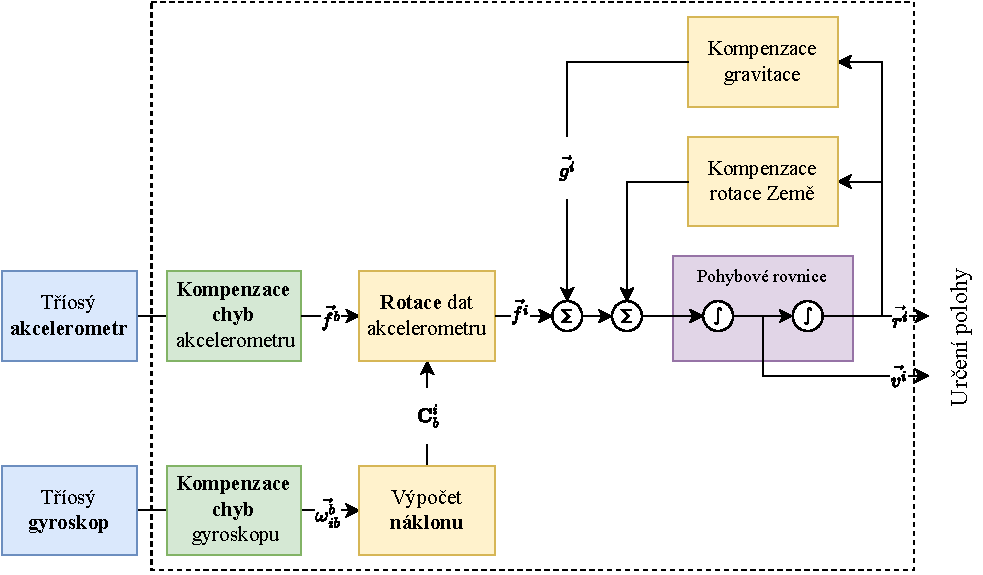
\includegraphics[width=0.85\columnwidth]{obrazky/StrapdownBlock}
				%lze vložit popisek, ale povetšinou je to v prezentaci zbytečné
				%\caption{Blokové schéma algoritmu strapdown inerciální navigace, převzato z [1] [2]}%
				%\label{obr:ukazka}
			\end{figure}
			\tiny [1] TITTERTON, D. H. a WESTON, J. L. \textit{Strapdown inertial navigation technology}. Second edition. Progress in astronautics and aeronautics, 207. Reston, VA: American Institute of Aeronautics and Astronautics, c2004. ISBN 1-56347-693-2.
	
\end{frame} 


%%%%%%%%%%%%%
\begin{frame} 
	\frametitle{Fúze dat z jiných senzorů}
		\begin{alertblock}{Nepřesnost}
		S časem díky integraci roste chyba měření.
		\end{alertblock}
		\vspace{4ex}
		\begin{block}{Možnosti snížení chyby}
		\begin{itemize}
		\item GNSS - při částečně dostupném signálu
		\item Magnetometr - omezení gyro driftu v horizontální rovině
		\end{itemize}
		\end{block}

	
\end{frame} 

%%%%%%%%%%%%%
\begin{frame} 
	\frametitle{Testování vývojových kitů}
	
	\begin{columns}[T] 								% prostředí sloupce s umístěním nahoře
		\begin{column}{0.3\textwidth}		% první sloupec
			3D tištěný držák pro zarovnání geometrických os:
			%
			\begin{itemize}
				\item IMU - ADIS16505
				\item GNSS - NEO-M8U
			\end{itemize}
			\vspace{0.5cm}
			Zpracování dat:
			%
			\begin{itemize}
				\item Matlab navigation toolbox - převážně pouze pro natočení, ne polohad
				\item Asynchronost USB komunikace
			\end{itemize}
		\end{column}
		%
		\begin{column}{0.7\textwidth}		% druhý sloupec
			\begin{figure}%	
				\centering
				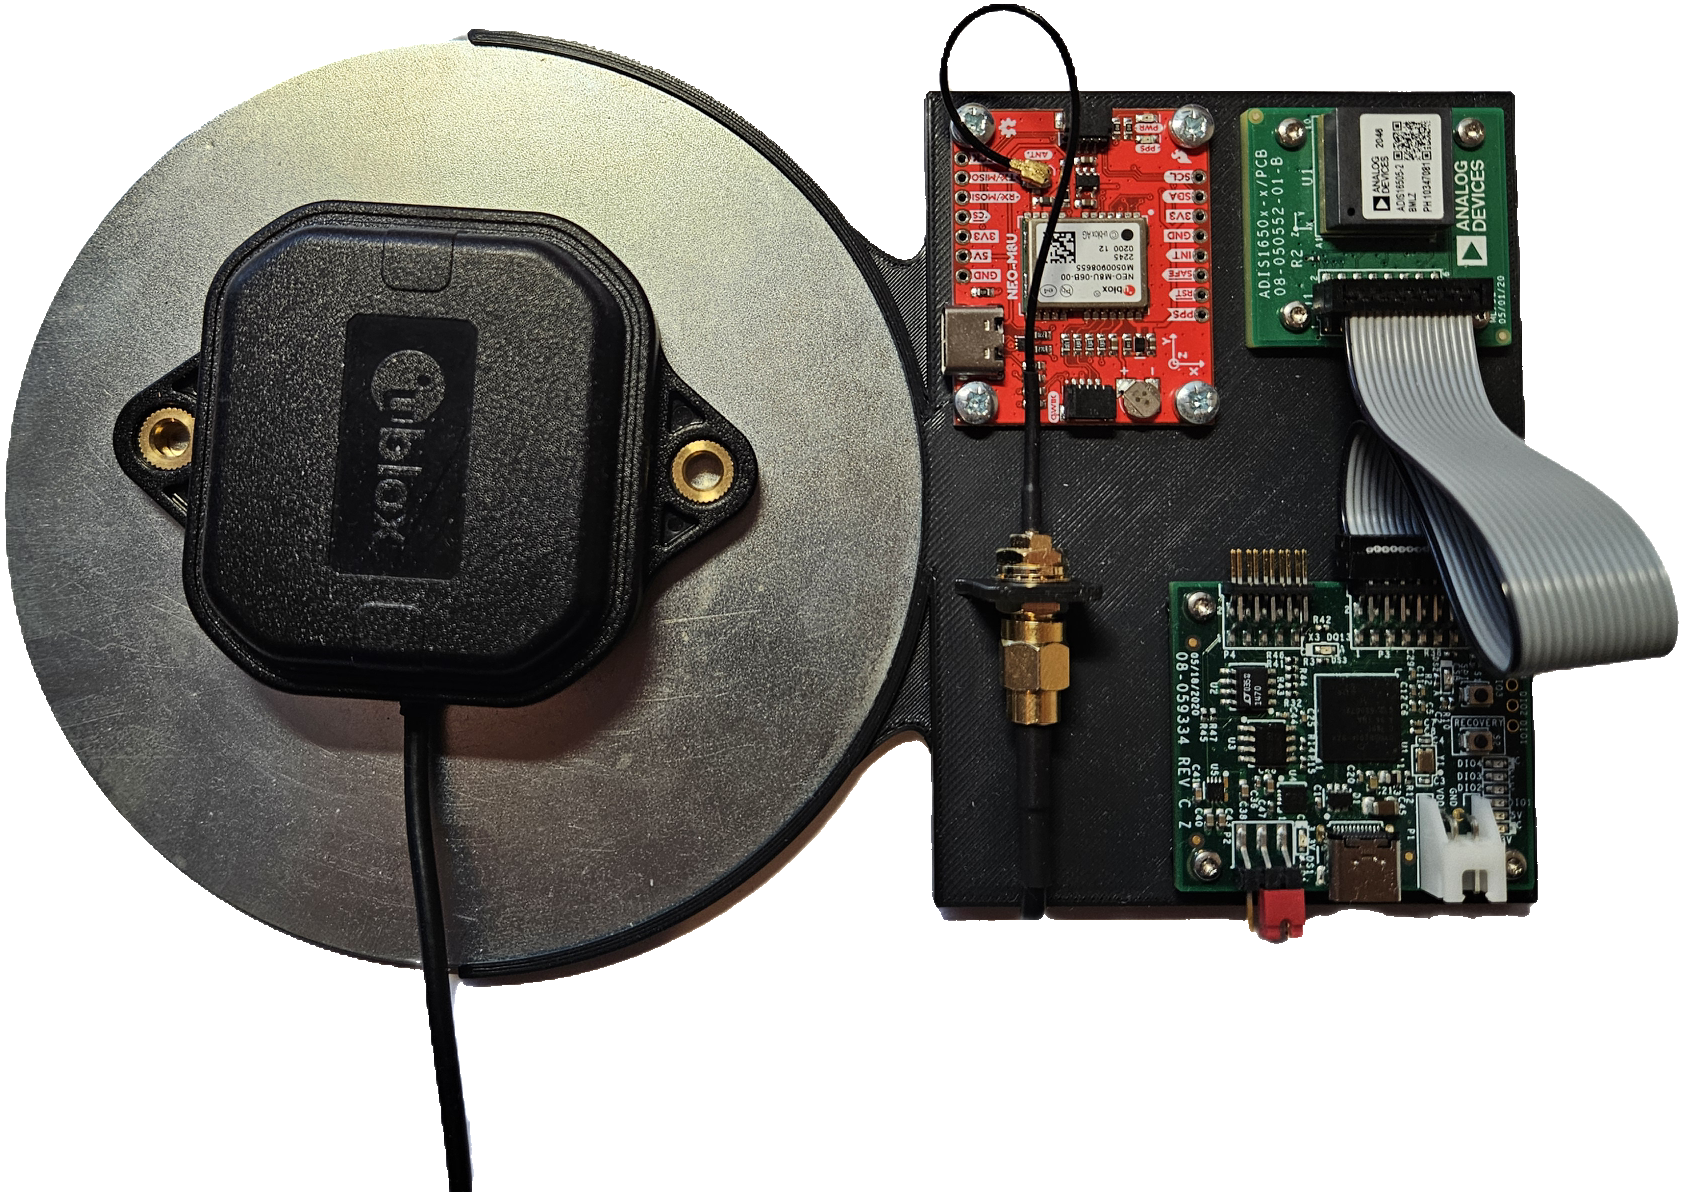
\includegraphics[width=1\columnwidth]{obrazky/devBoards}
				%lze vložit popisek, ale povetšinou je to v prezentaci zbytečné
				%\caption{Testovací přípravek s vývojovými deskami}%
				%\label{obr:ukazka}
			\end{figure}
		\end{column}
	\end{columns}						
			

	
\end{frame} 

%%%%%%%%%%%%%
\begin{frame} 
	\frametitle{Hardware inerciální jednotky}
	
			\begin{figure}%	
				\centering
				
				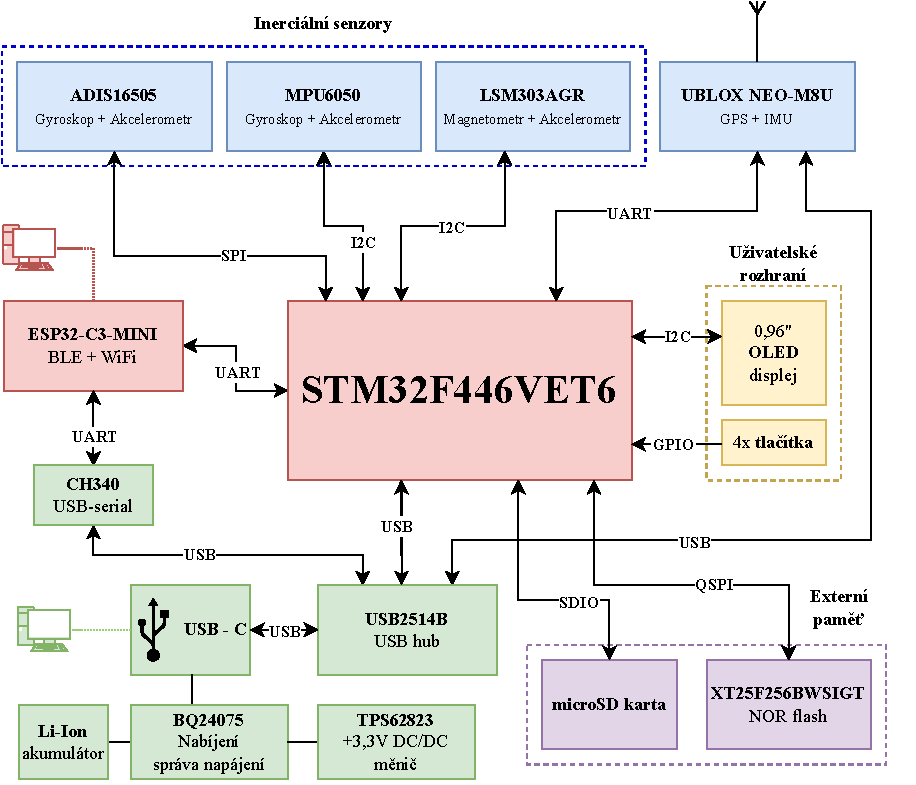
\includegraphics[width=0.62\columnwidth]{obrazky/IMUnav_H00_block}
				%lze vložit popisek, ale povetšinou je to v prezentaci zbytečné
				%\caption{Blokové schéma inerciální jednotky}%
				%\label{obr:ukazka}
			\end{figure}
	
\end{frame} 




%%%%%%%%%%%%%
\begin{frame} 
	\frametitle{Požadavky na paměť}
	\begin{table}[h!]
\centering
\begin{tabular}{c|c}

Senzor & Odhadovaný bitrate \\ 
\hline 
\hline 
ADIS16505-2 & 375 kbit/s \\ 

MPU-6050 & 422 kbit/s \\ 

LSM303AGR & 7 kbit/s \\ 

NEO-M8U & 1 kbit/s \\ 
\hline

Celkem & 805 kbit/s (0,1MB/s) \\ 

\end{tabular} 
%\caption{Odhad celkového bitratu pro záznam dat} 
\label{table:memoryBW}
\end{table} 
	
	12 MB dat při dvouminutovém záznamu.
	
	\begin{itemize}
	\item SD karta
	\item 32 MB NOR Flash
	\end{itemize}
	
\end{frame} 


%%%%%%%%%%%%%
\begin{frame} 
	\frametitle{Plošný spoj}
	
	\begin{columns}[T] 								% prostředí sloupce s umístěním nahoře
		\begin{column}{0.4\textwidth}		% první sloupec
			
			\begin{itemize}
				\item KiCad
				\item Čtyřvrstvá deska $ 100 \times 100$ mm
				\item Impedance vedení pro GNSS a USB
				\item hřebínky na odposlech komunikací
			\end{itemize}
		\end{column}
		%
		\begin{column}{0.6\textwidth}		% druhý sloupec
			\begin{figure}%	
				\centering
			    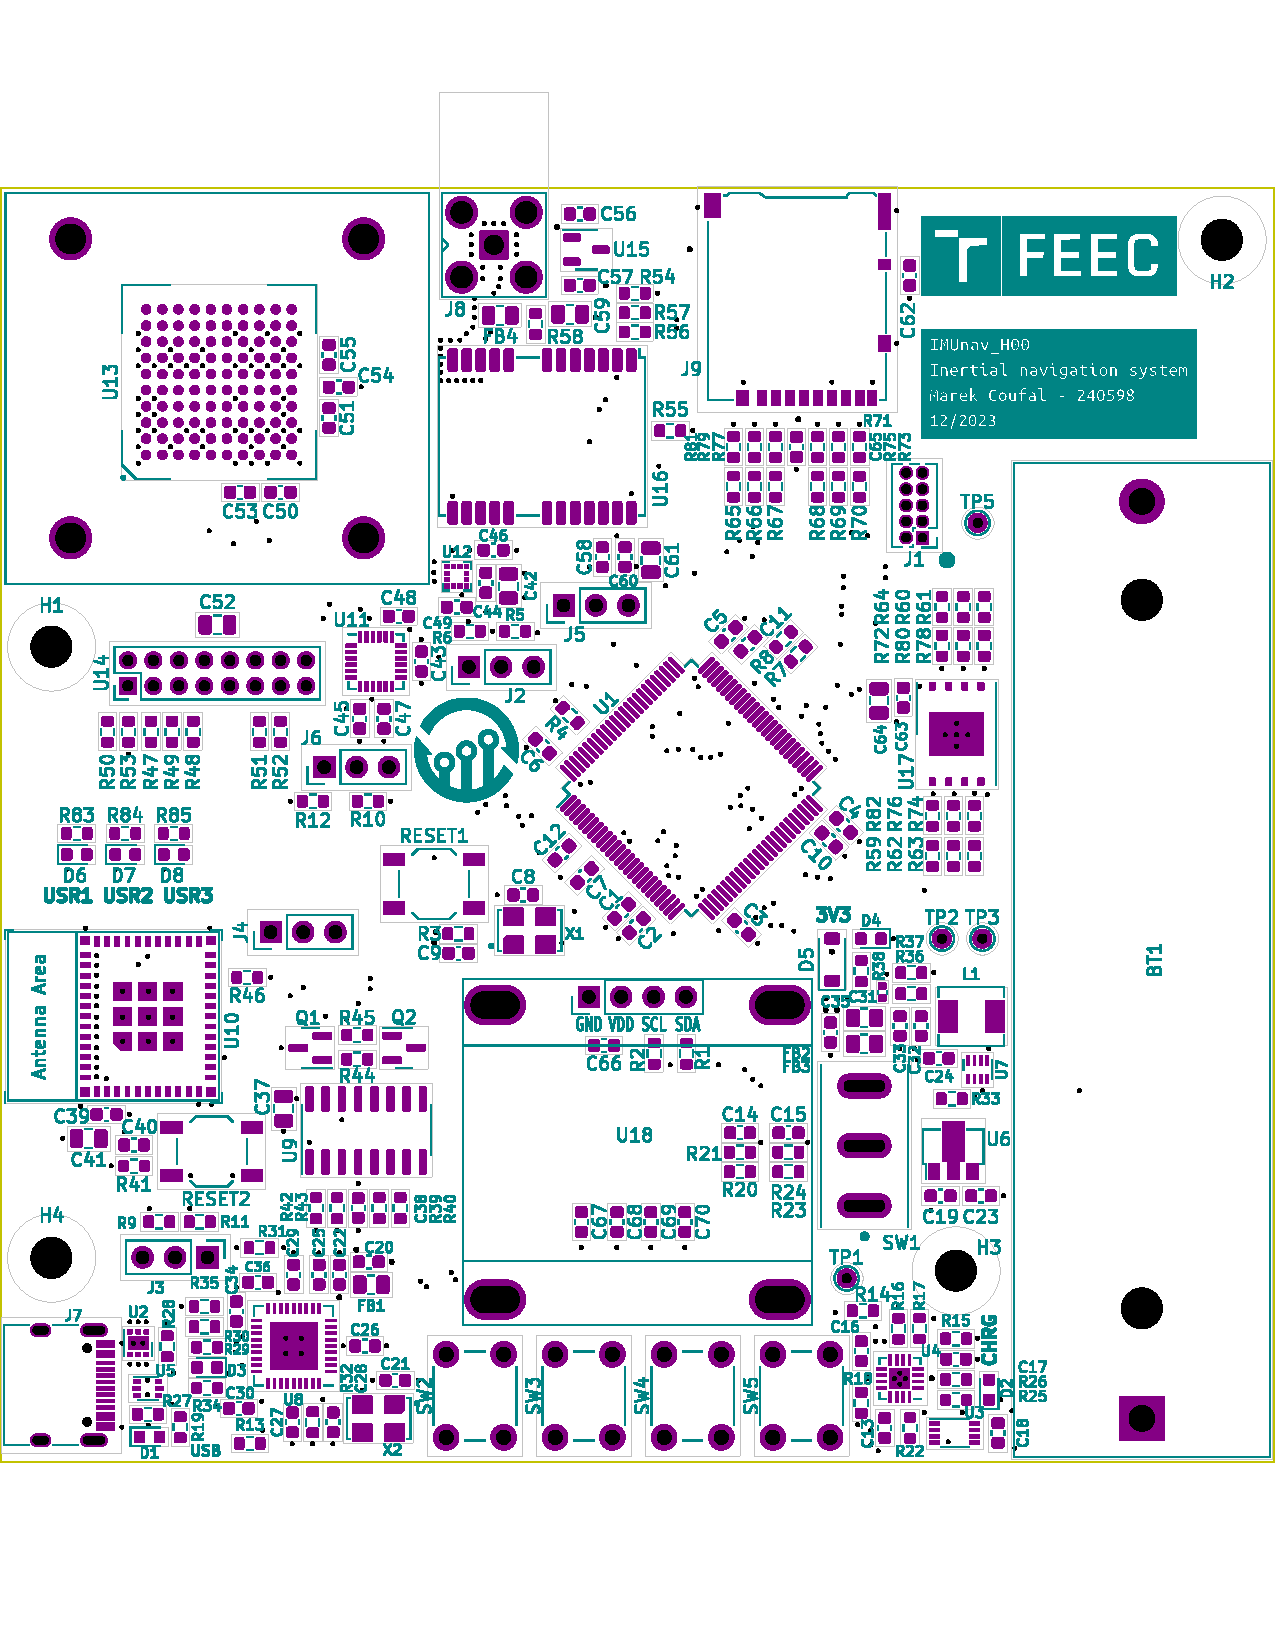
\includegraphics[width=0.78\columnwidth, trim={0 3.2cm 0 1.5cm},clip]{KiCad/boardTopParts}
				%lze vložit popisek, ale povetšinou je to v prezentaci zbytečné
				%\caption{Pohled osazení součástek}%
				%\label{obr:ukazka}
			\end{figure}
		\end{column}
	\end{columns}											% ukončení prostředí sloupce
\end{frame}




%%%%%%%%%%%%%
\begin{frame} 
	\frametitle{3D modely}
	\begin{columns}[T] 								% prostředí sloupce s umístěním nahoře
		\begin{column}{0.5\textwidth}		% první sloupec
		\begin{figure}%
		\centering
		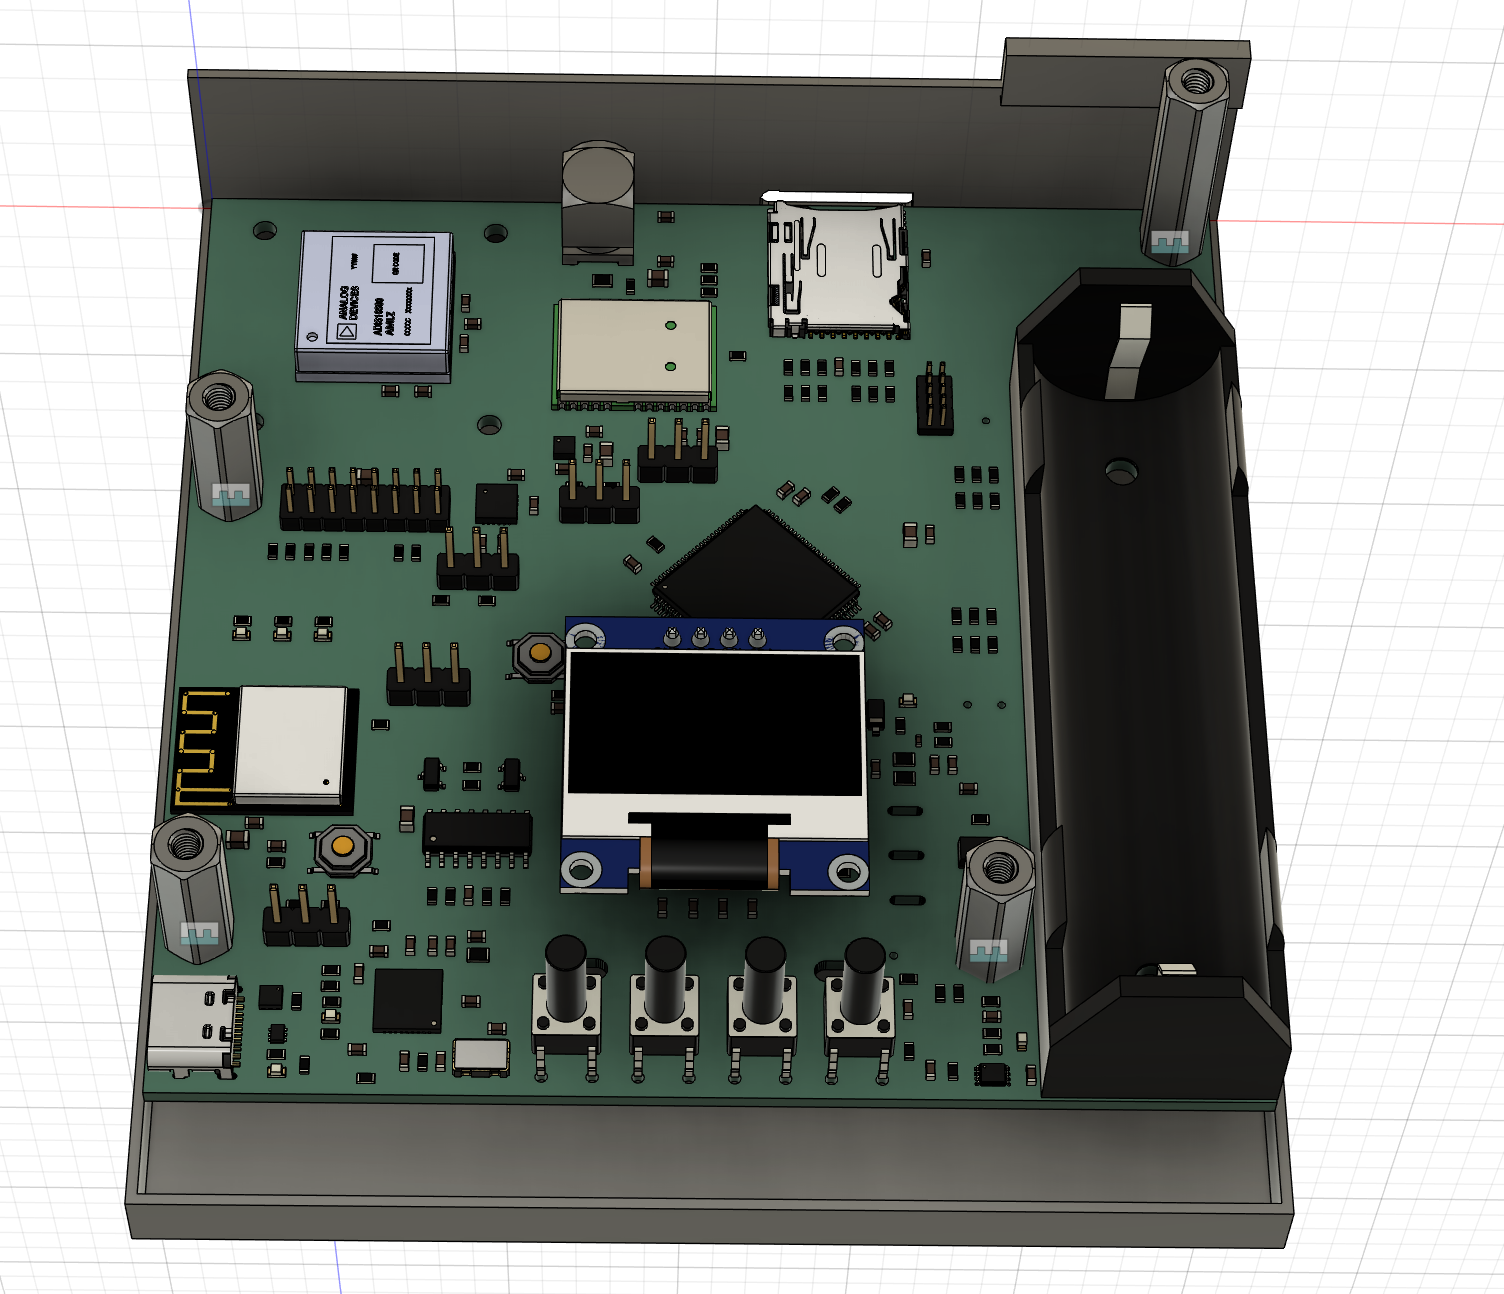
\includegraphics[width=1\columnwidth]{obrazky/boxNoLid}
		\end{figure}
		\end{column}
		%
		\begin{column}{0.5\textwidth}		% druhý sloupec
		\begin{figure}%
		\centering
		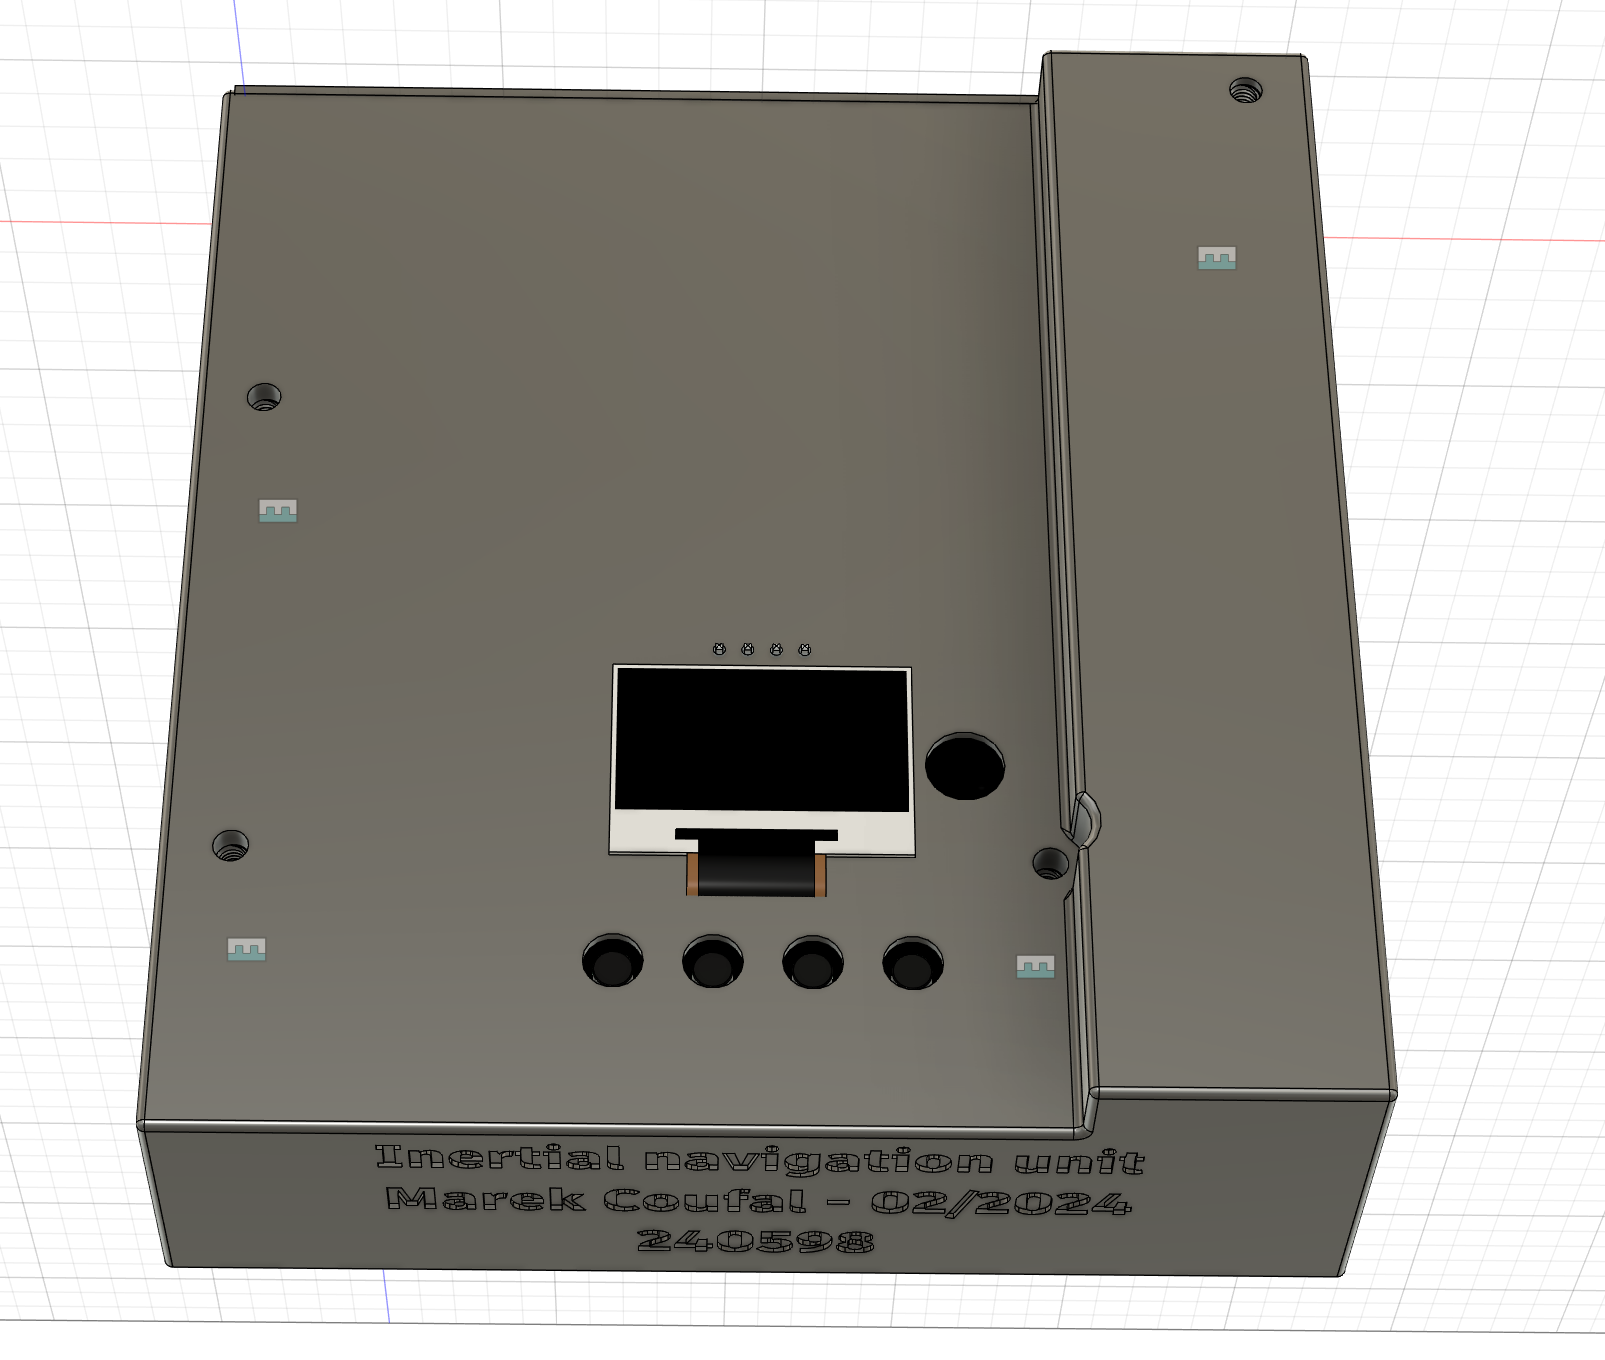
\includegraphics[width=1\columnwidth]{obrazky/boxWithLid}
		\end{figure}
		\end{column}
	\end{columns}	
\end{frame}

%%%%%%%%%%%%%
\begin{frame} 
	\frametitle{Sestavené zařízení}
	\begin{columns}[T] 								% prostředí sloupce s umístěním nahoře
		\begin{column}{0.5\textwidth}		% první sloupec
		\begin{figure}%
		\centering
		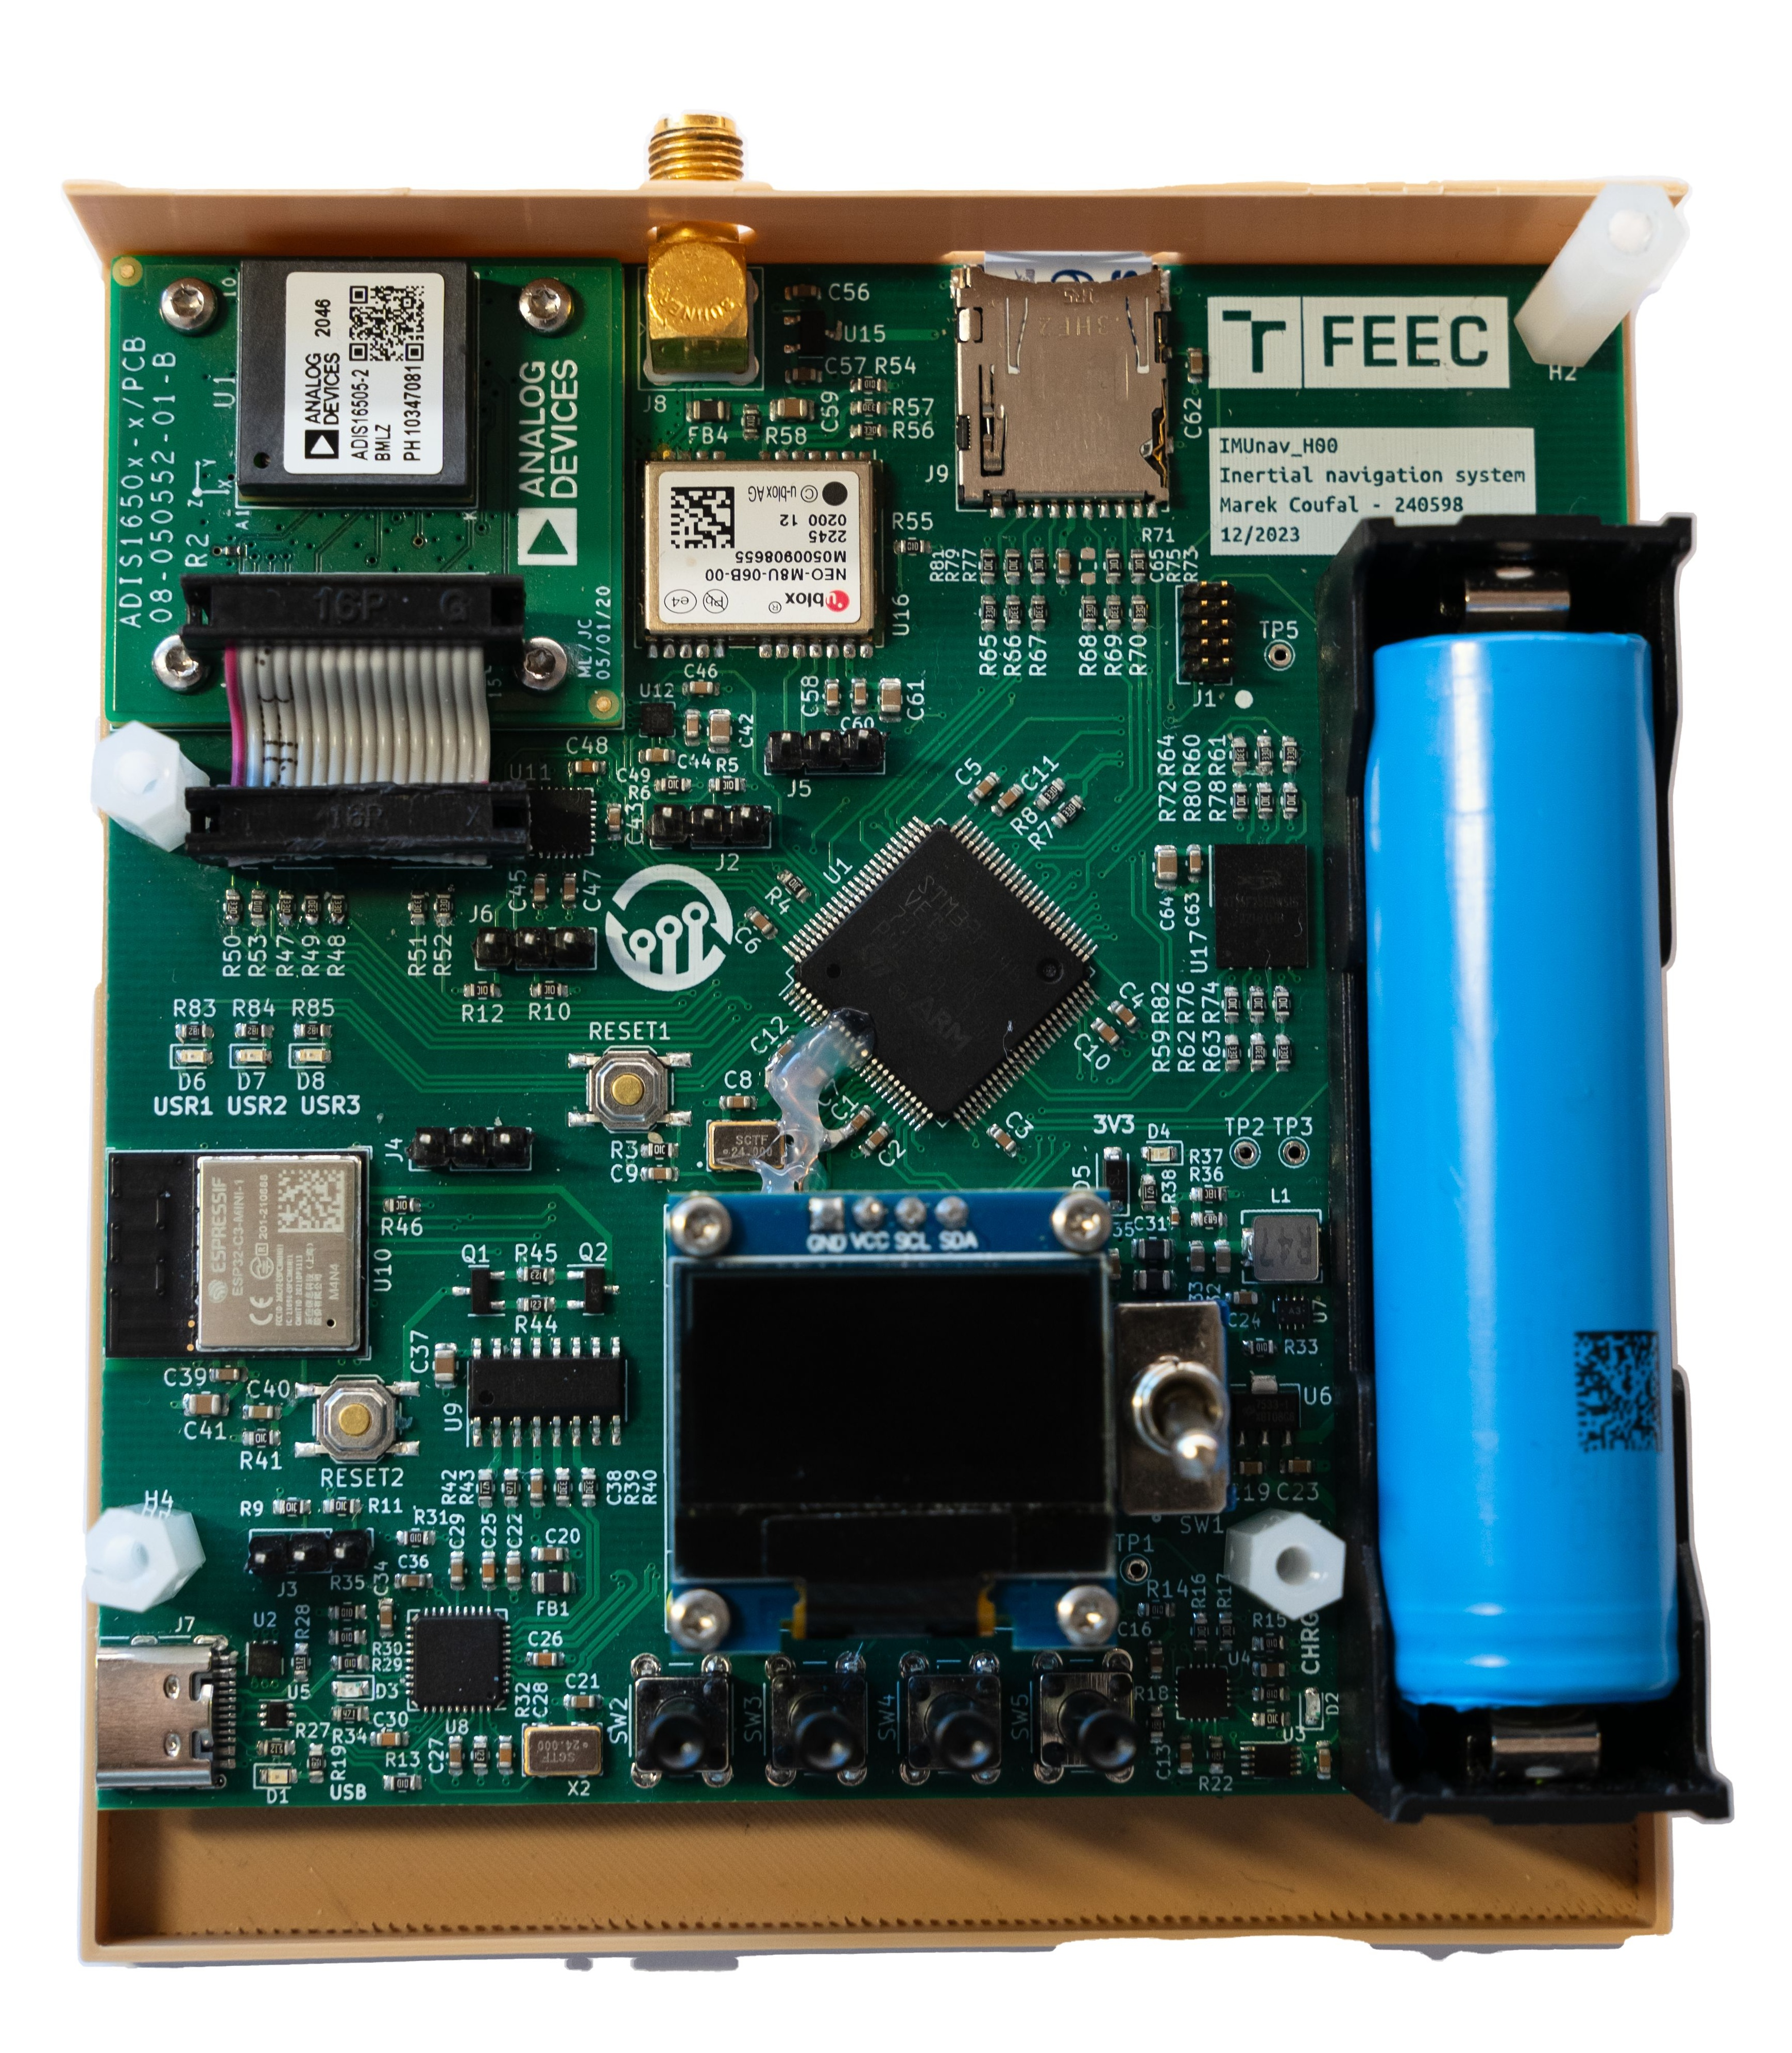
\includegraphics[width=0.9\columnwidth]{obrazky/imuNavPCB}
		\end{figure}
		\end{column}
		%
		\begin{column}{0.5\textwidth}		% druhý sloupec
		\begin{figure}%
		\centering
		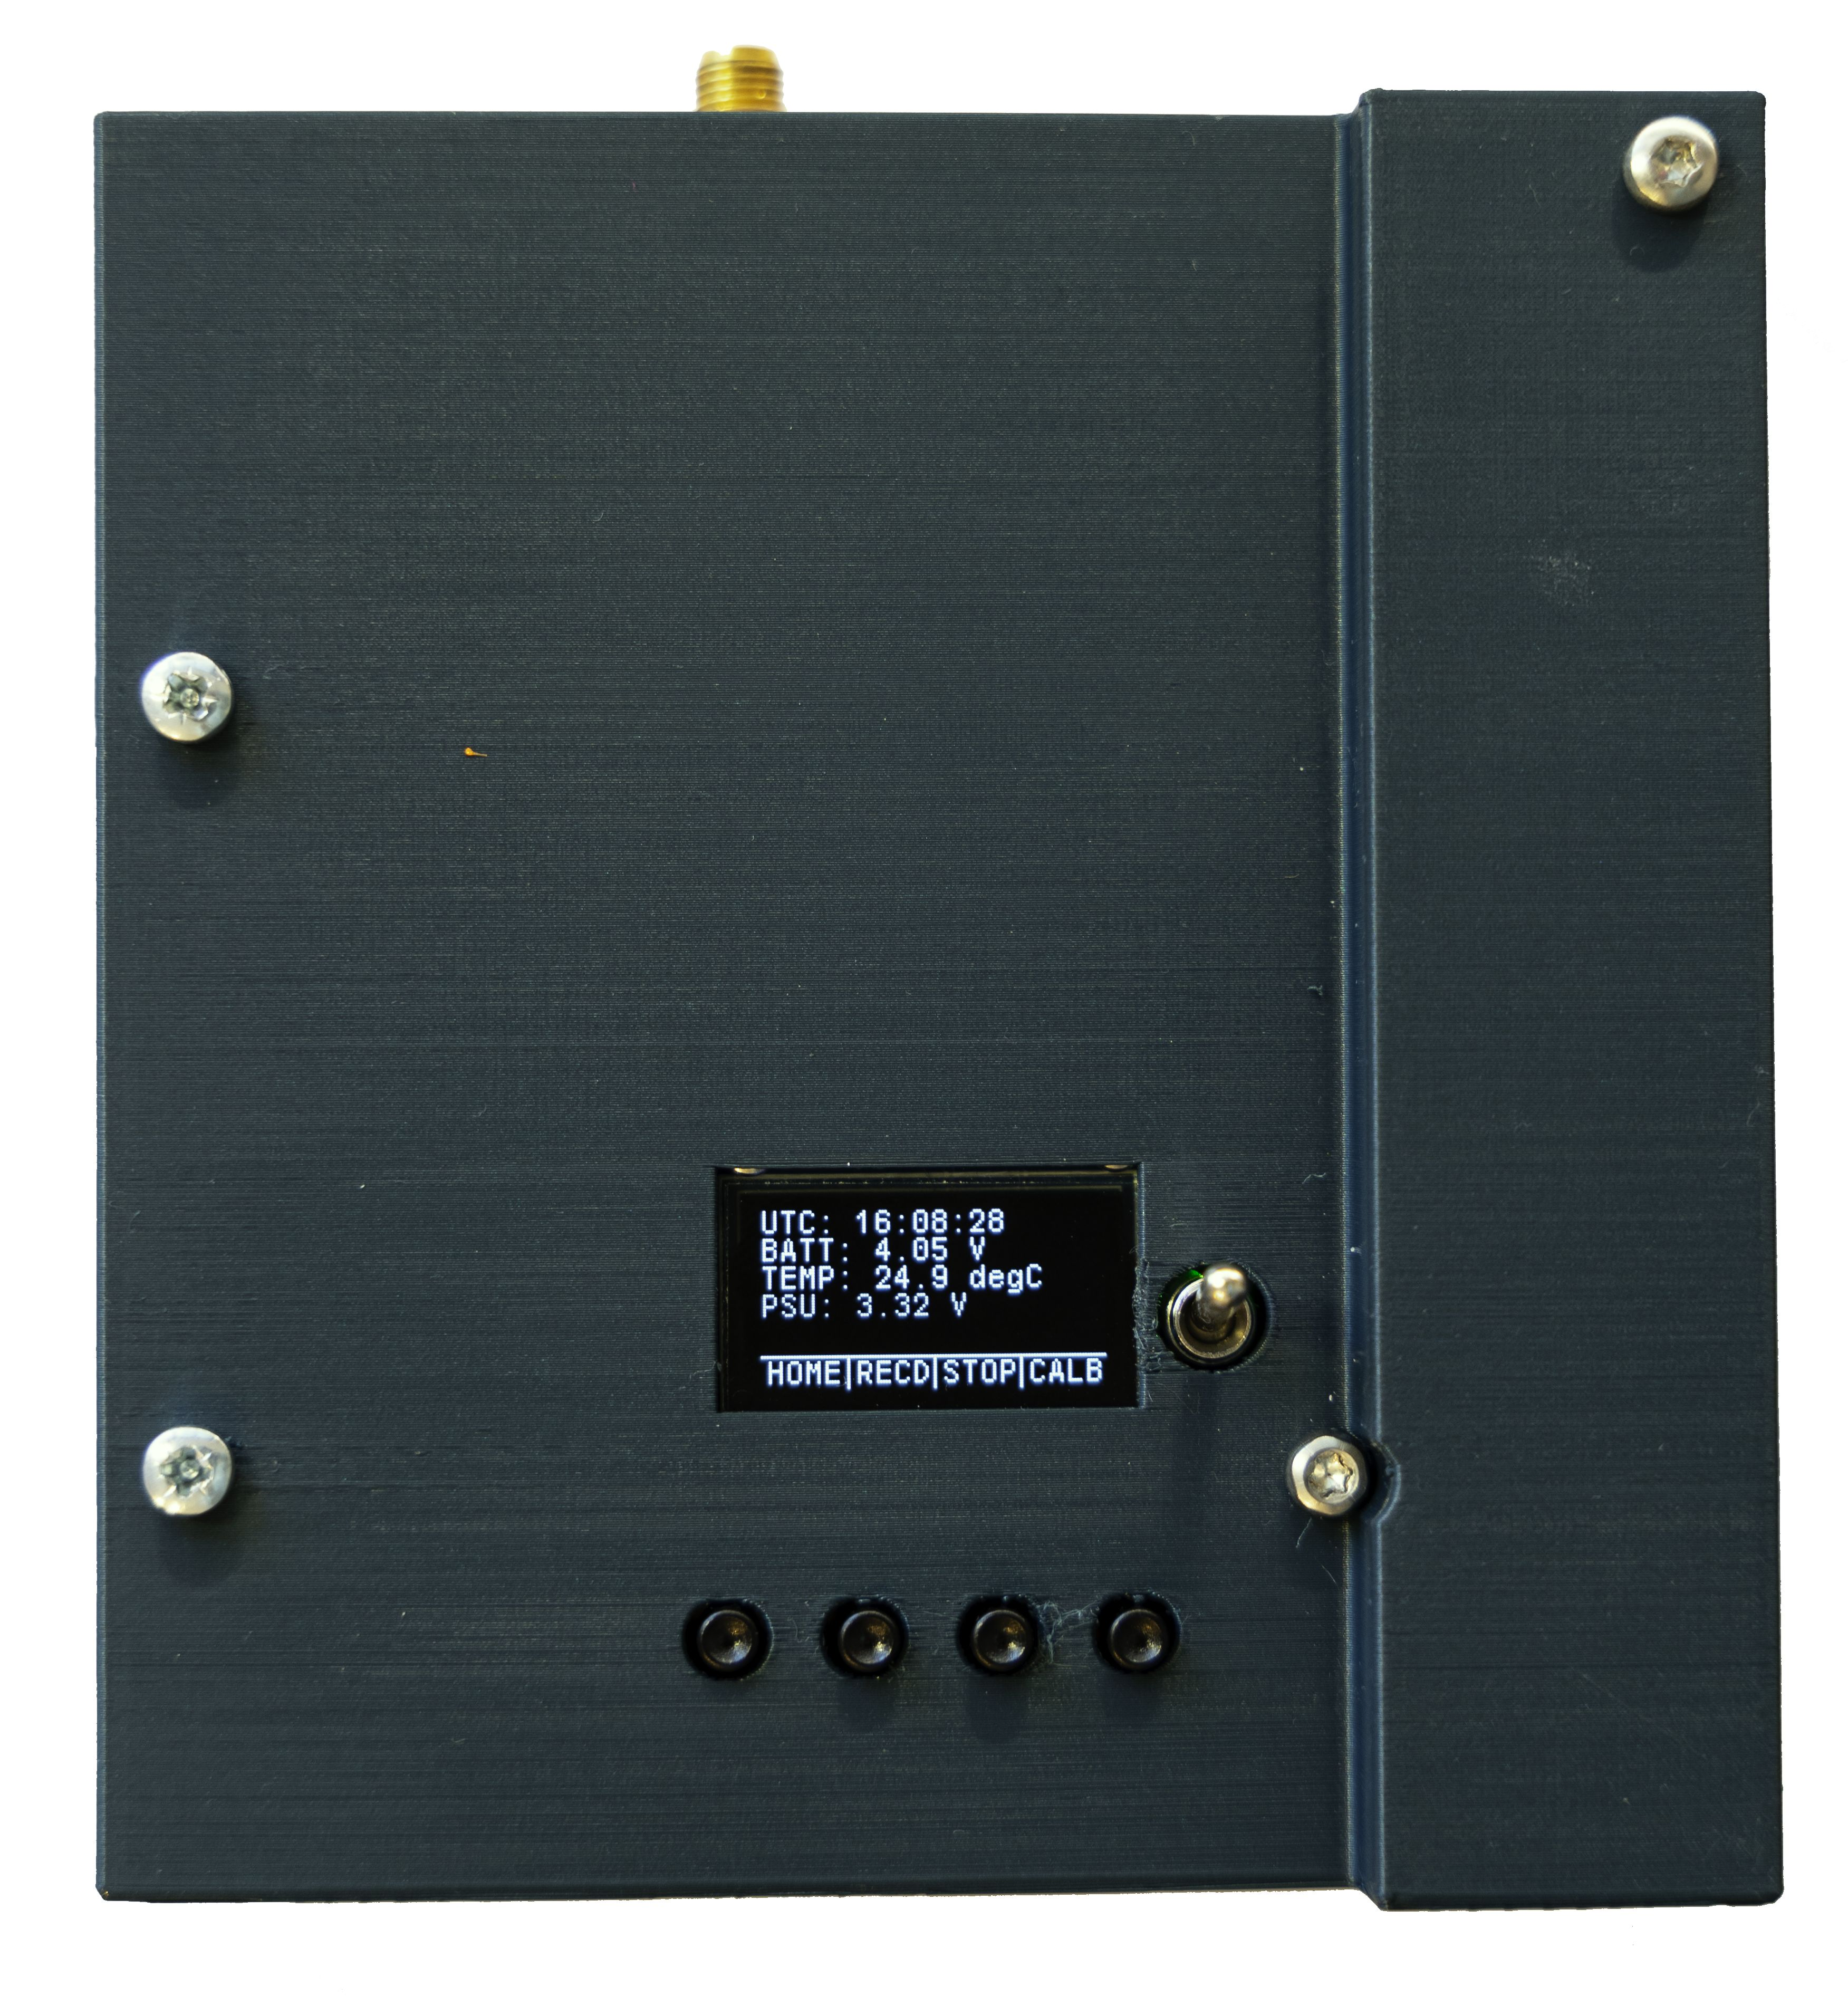
\includegraphics[width=0.9\columnwidth]{obrazky/ImunavFront}
		\end{figure}
		\end{column}
	\end{columns}	
\end{frame}

%%%%%%%%%%%%%
\begin{frame} 
	\frametitle{Firmware}
	
	\begin{columns}[T] 								% prostředí sloupce s umístěním nahoře
		\begin{column}{0.5\textwidth}		% první sloupec
			
			\begin{itemize}
				\item STM32CubeIDE
				\item HAL
				\item FreeRTOS
				\item FatFS, USB Mass Storage Class
				\item Grafické rozhraní, tlačítka
				\item Zobrazení aktuálních hodnot
				\item Záznam dat
				\item Kalibrace IMU pomocí MATLAB Coder
				\item Převod dat z binární podoby do CSV pomocí Pythonu/
				
				
			\end{itemize}
		\end{column}
		%
		\begin{column}{0.25\textwidth}		% druhý sloupec
			\begin{figure}%	
				\centering
			    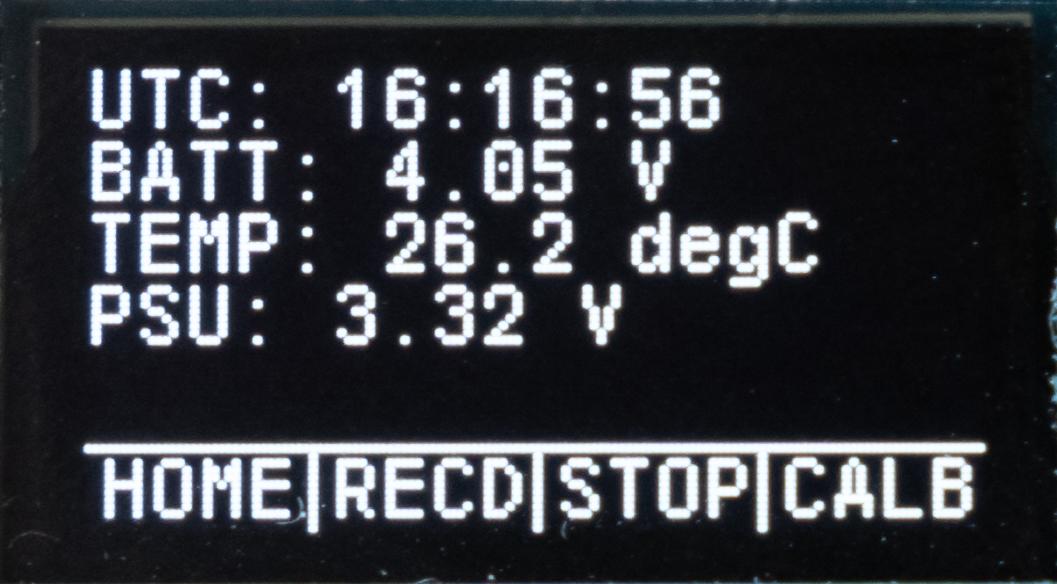
\includegraphics[width=1\columnwidth]{obrazky/menuHome}
			\end{figure}
			\begin{figure}%	
				\centering
			    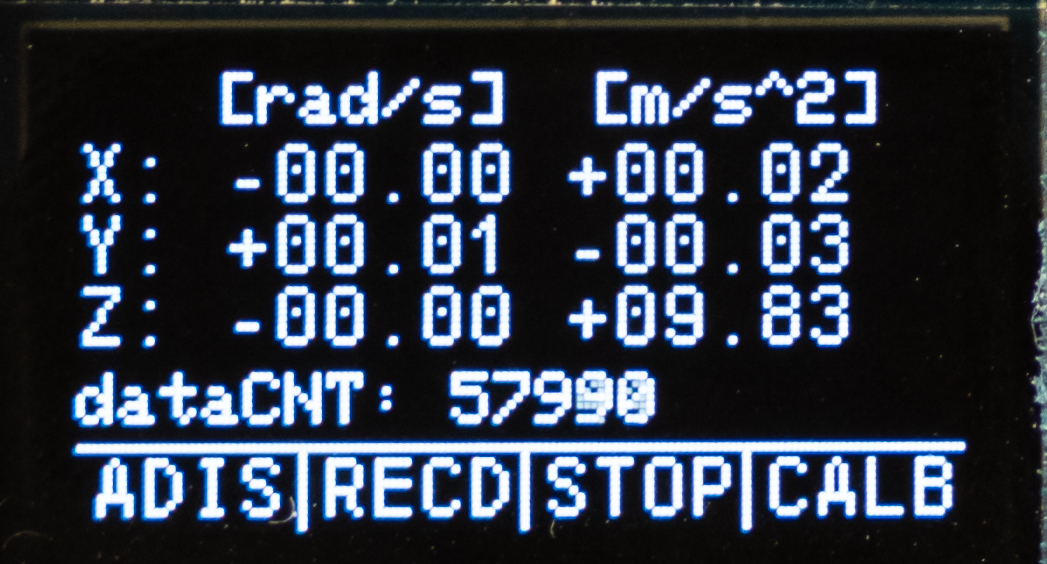
\includegraphics[width=1\columnwidth]{obrazky/menuADIS}
			\end{figure}
			\begin{figure}%	
				\centering
			    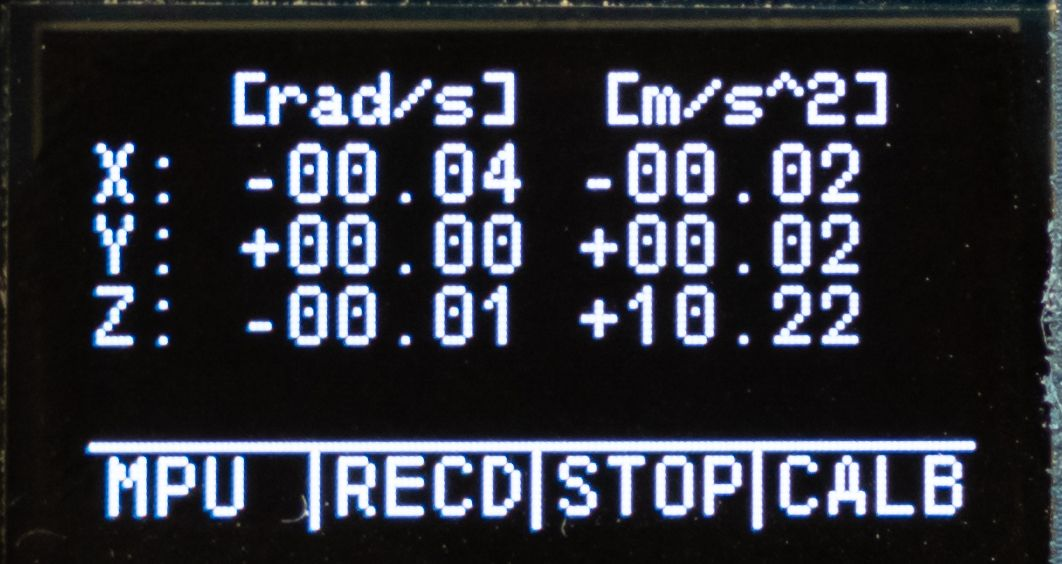
\includegraphics[width=1\columnwidth]{obrazky/menuMPU}
			\end{figure}

		\end{column}
		
				\begin{column}{0.25\textwidth}		% druhý sloupec
			\begin{figure}%	
				\centering
			    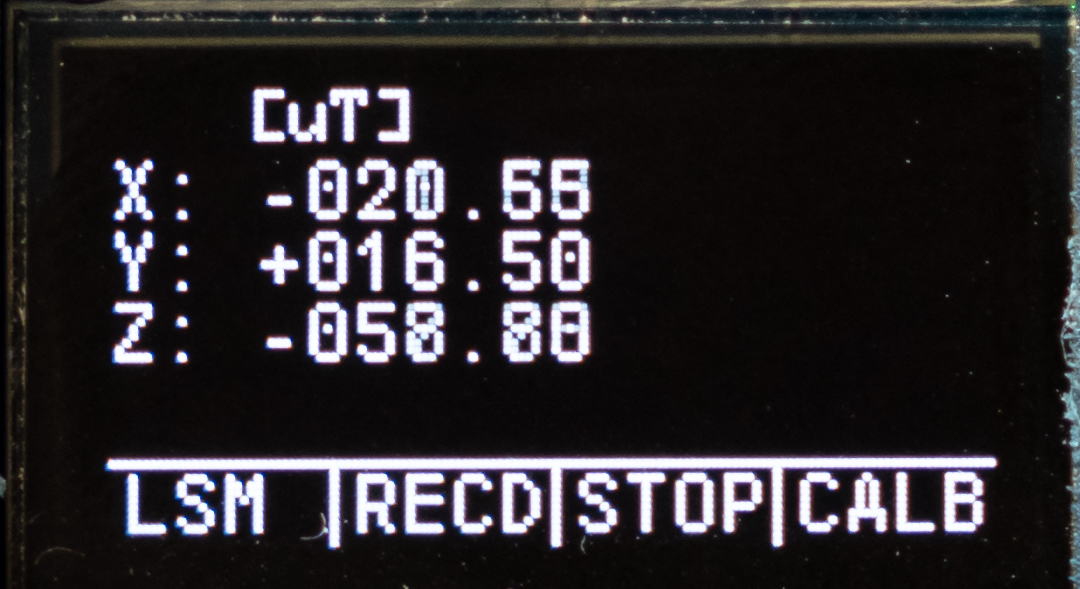
\includegraphics[width=1\columnwidth]{obrazky/menuLSM}
			\end{figure}
			\begin{figure}%	
				\centering
			    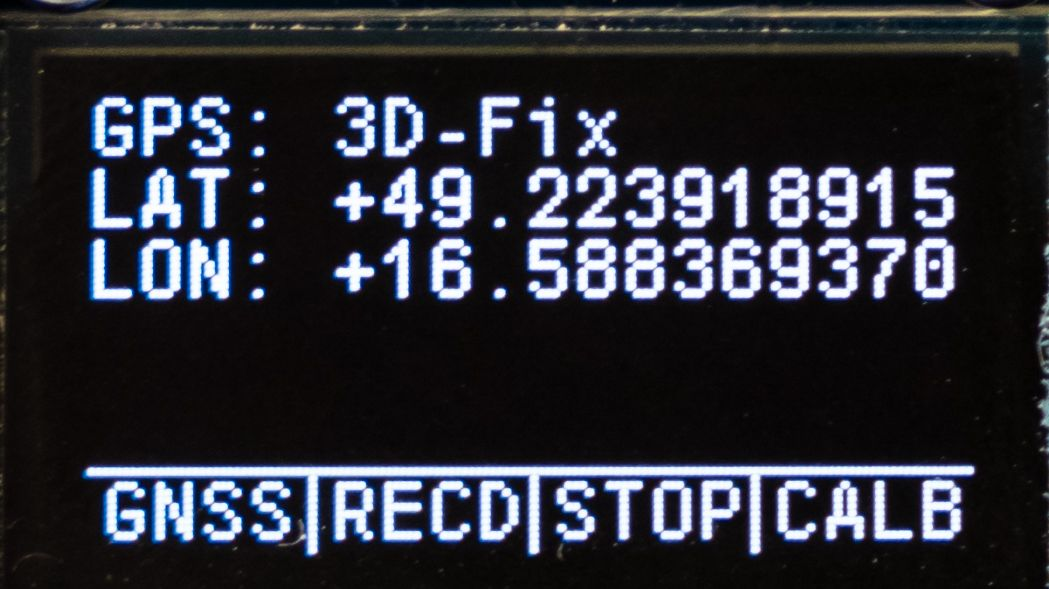
\includegraphics[width=1\columnwidth]{obrazky/menuGPS}
			\end{figure}
			\begin{figure}%	
				\centering
			    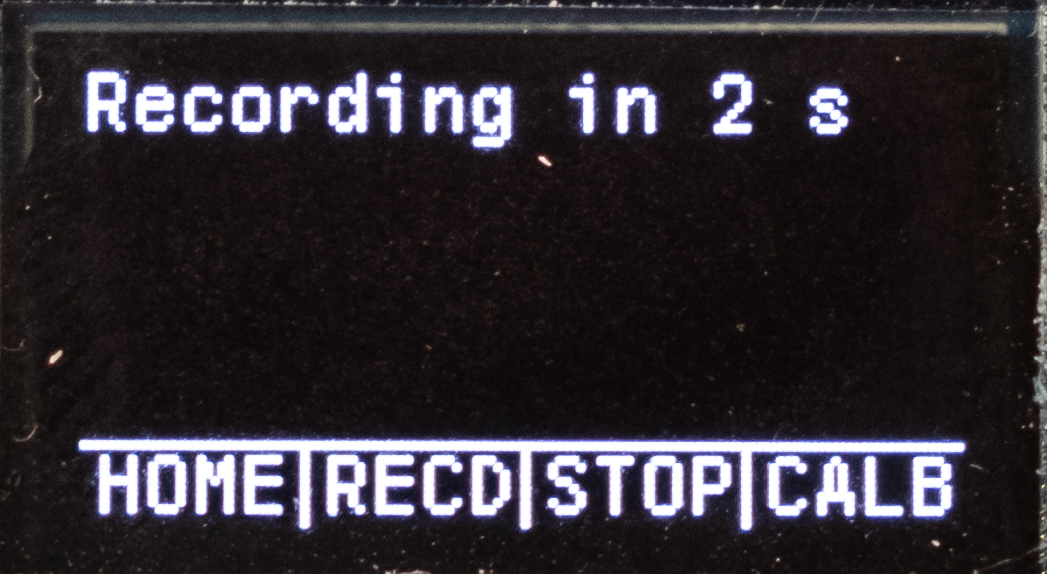
\includegraphics[width=1\columnwidth]{obrazky/menuREC1}
			\end{figure}
			\end{column}

	\end{columns}											% ukončení prostředí sloupce
\end{frame}

%%%%%%%%%%%%%
\begin{frame} 
	\frametitle{Software - čistě inerciální navigace - naměřená data}
	\begin{columns}[T] 								% prostředí sloupce s umístěním nahoře
		\begin{column}{0.5\textwidth}		% první sloupec
		\begin{figure}%
		\centering
		\includegraphics[width=1\columnwidth]{obrazky/matlab/1measAccel-eps-converted-to}
		\end{figure}

		\end{column}
		%
		\begin{column}{0.5\textwidth}		% druhý sloupec
		\begin{figure}%
		\centering
		\includegraphics[width=1\columnwidth]{obrazky/matlab/1measAngularVel-eps-converted-to}
		\end{figure}
		\end{column}
	\end{columns}	
\end{frame}

%%%%%%%%%%%%%
\begin{frame} 
	\frametitle{Software - čistě inerciální navigace - integrace}
	\begin{columns}[T] 								% prostředí sloupce s umístěním nahoře
		\begin{column}{0.5\textwidth}		% první sloupec
		\begin{figure}%
		\centering
		\includegraphics[width=1\columnwidth]{obrazky/matlab/1measOrient-eps-converted-to}
		\end{figure}

		\end{column}
		%
		\begin{column}{0.5\textwidth}		% druhý sloupec
		\begin{figure}%
		\centering
		\includegraphics[width=1\columnwidth]{obrazky/matlab/1measAccelEframeWithoutG-eps-converted-to}
		\end{figure}
		\end{column}
	\end{columns}	
\end{frame}

%%%%%%%%%%%%%
\begin{frame} 
	\frametitle{Software - čistě inerciální navigace - výsledek}
	\begin{columns}[T] 								% prostředí sloupce s umístěním nahoře
		\begin{column}{0.5\textwidth}		% první sloupec
		\begin{itemize}
				\item Velká chyba
				
				
			\end{itemize}

		\end{column}
		%
		\begin{column}{0.5\textwidth}		% druhý sloupec
		\begin{figure}%
		\centering
		\includegraphics[width=1\columnwidth]{obrazky/matlab/1measTraj-eps-converted-to}
		\end{figure}
		\end{column}
	\end{columns}	
\end{frame}


% podekovani
\begin{frame}[c] 
% bez nadpisu snímku
	\frametitle{\mbox{ }}
	\begin{center}
		{\Huge Děkuji za pozornost!}
	\end{center}
\end{frame}


\end{document}
